\documentclass[11pt]{article}

\usepackage{amsmath}
\usepackage{amssymb,latexsym}
\usepackage{amsthm}
\usepackage[spanish]{babel}
\usepackage[pdftex]{graphicx} % PDFLaTeX
\DeclareGraphicsExtensions{.png,.pdf,.jpg}
\usepackage{epsf}
\usepackage{graphicx}

\newtheorem{teorema}{Teorema}[section]
\newtheorem{lema}[teorema]{Lema}
\theoremstyle{definition}
\newtheorem{definicion}[teorema]{Definici\'on}
\newtheorem{problema}{Problema}
\newtheorem{ejemplo}{Ejemplo}

\renewcommand{\baselinestretch}{1.2}
\usepackage[bottom]{footmisc}  % places footnotes at page bottom
\usepackage[latin1]{inputenc}      %    tipo de codificacion del documento: applemac,

\usepackage{subfigure}
%\usepackage{hyperref}
%\usepackage[pdftitle={},pdfauthor={}, colorlinks=true, hyperindex=true, linkcolor=blue, pdfpagemode=UseOutlines, bookmarksopen=false, bookmarksnumbered=true, pdfstartview={FitH}]{hyperref} % %backref={page} para referencia de pagina
\spanishdecimal{.}
\usepackage{amssymb,amsmath,latexsym,amsfonts}
\usepackage{rotating}
\usepackage{indentfirst}        %
%\usepackage[]{showkeys}

\begin{document}

\title{C�LCULO PARA EL AN�LISIS ECON�MICO}
\author{\textbf{ESCUELA SUPERIOR DE ECONOM�A}}
\date{\large{M\'exico, D.F., 27 de Agosto de 2010}}
\def\contentsname{Contenido}

\newpage

\setcounter{page}{1}

\section{Derivadas}

\section{Optimizaci�n libre con una variable}

\section{C�lculo en varias variables}

\newpage

\section{Optimizaci\'on libre y restringida en varias \\
         va\-ria\-bles}

\textbf{Introducci\'on}
\medskip

Los problemas de optimizaci\'on se pueden describir usualmente  de
la siguiente forma matem\'atica. Hay una \textbf{funci\'on objetivo}
$f(x_1,...,x_n)$, que es una funci\'on real de $n$ variables  de la
que hay que hallar los valores m\'aximos o m\'{\i}nimos. Tambi\'en
hay un \textbf{conjunto de restricciones} o un \textbf{conjunto de
oportunidades} $S$ que es un subconjunto de $\Bbb{R}^{n}.$

\vspace{.2cm}

Se pueden abarcar varios tipos de distintos problemas de
optimizaci\'on dando el conjunto $S$ adecuadamente. Si $f$ tiene un
punto \'optimo en el interior de $S$ se habla del caso cl\'asico. Si
$S$ es el conjunto  de todos los puntos $(x_1,...,x_n)$ que
verifican un cierto n\'umero de ecuaciones tenemos un problema
lagrangiano, que es maximizar o minimizar una funci\'on  sujeta a
restricciones de igualdad.


\subsection{Optimizaci�n libre}

Sea $f$ una funci\'on de $n$ variables $x_1,...,x_n$ definida en un dominio
 $S \subset \Bbb{R}^{n}$. Sea $c = (c_1,...,c_n) \in S$ y supongamos que $f$ toma
 un valor  en $c$ que es mayor o igual que todos los valores de $f$ en los otros puntos
 $x = (x_1,...,x_n)$ de $S$, es decir:
 \[
     f(x) \leq f(c) \,\, \text{para todo} \,\,  x   \in S.
 \]
Entonces se llama a $c$ un \textbf{ m\'aximo global} de $f$ en $S$ y
a $f(c)$ el \textbf{ va\-lor m\'aximo}. De forma an\'aloga definimos
un \textbf{ m\'{\i}nimo global} y el \textbf{valor m\'{\i}nimo}
invirtiendo el signo de la desigualdad. Conjuntamente se usar\'an
los nombres de \'optimos y valores \'optimos para significar
m\'aximos o m\'{\i}nimos. El vector $c$ se llama \textbf{ un punto
estacionario} de $f(x_1,...,x_n)$ si $x = c$ es una soluci\'on  de
las $n$ ecuaciones:
\[
\frac{\partial f}{\partial x_1 } (x) = 0, \,\,   \frac{\partial f}{\partial x_2 } (x) = 0,...,\,\,
\frac{\partial f}{\partial x_n } (x) = 0,
\]

\begin{teorema}
Sea $f$ una funci\'on  definida en un conjunto $S \subset
\Bbb{R}^{n}$ y sea $c= (c_1,...,c_n)$ un punto interior de $S$ en el
que $f$ es diferenciable. Una condici\'on necesaria para que $c$ sea
un m\'aximo o un m\'{\i}nimo
 para $f$ es que $c$ sea un punto estacionario para $f$, es decir,
 \[
    f'_i(c) = 0 \,\, (i = 1,...,n).
 \]
En particular se tiene el siguiente
\end{teorema}

\begin{teorema}
\label{porden} Una condici\'on necesaria para que una funci\'on
$f(x,y)$ di\-fe\-ren\-cia\-ble tenga un m\'aximo o un m\'{\i}nimo en
un punto interior $(x_0,y_0)$ de su dominio es que $(x_0,y_0)$ sea
un punto estacionario de $f$, esto es,

\begin{equation}
        f_x'(x_0,y_0) =  0,\,\, f_y'(x_0,y_0) = 0.
\end{equation}
\end{teorema}

\begin{teorema}
\label{soptimos} (Condiciones suficientes de \'optimos globales) Si
$f(x,y)$ es una funci\'on con derivadas parciales primeras y
segundas continuas en un dominio convexo $S$, y sea $(x_0, y_0)$ un
punto estacionario de $f$ interior a $S$, entonces la condici\'on
suficiente para que la funci\'on $f(x,y)$
 tenga un m\'aximo o un m\'{\i}nimo respectivamente es:

\vspace{.2cm}

\begin{enumerate}
 \item[(a)] Si para todo $(x, y) \in S$ se cumplen las siguientes condiciones:
  \[
  D(x,y)=f_{xx}''(x,y)f_{yy}''(x,y) - [f_{xy}''(x,y)]^{2} < 0,
  \]
  entonces $(x_0, y_0)$ es un punto de silla de $f(x,y)$ en $S$.

  \item[(b)] Si para todo $(x, y) \in S$ se cumplen las siguientes condiciones:
\[
  D(x,y) = f_{xx}''(x,y)f_{yy}''(x,y) - [f_{xy}''(x,y)]^{2} >0,\,\, \text{y}\,\,
  f_{xx}''(x,y) < 0,
\]
  entonces $(x_0, y_0)$ es un m\'aximo de $f(x,y)$ en $S$.

  \item[(c)] Si para todo $(x, y) \in S$ se cumplen las siguientes condiciones:
  \[
  D(x,y)=f_{xx}''(x,y)f_{yy}''(x,y) - [f_{xy}''(x,y)]^{2} > 0, \,\, \text{y}  \,\,
  f_{xx}''(x,y) > 0,
  \]
 entonces $(x_0, y_0)$ es un m\'{\i}nimo de $f(x,y)$ en $S$.
\end{enumerate}
\end{teorema}

\begin{ejemplo}
Encuentre todos los puntos  cr\'{\i}ticos de la funci\'on $f(x,y) =
x^2 + y^2$ y clasifique cada uno como un m\'aximo relativo, un
m\'{\i}nimo relativo o un punto de silla.


\vspace{.2cm}

\textbf{Soluci\'on}

Como
\[
    f_x = 2x \quad  \text{y} \quad f_y = 2y
\]
el \'unico punto cr\'{\i}tico de $f$ es $(0,0)$. Para poner a prueba
este punto, use las derivadas parciales de segundo orden
\[
   f_{xx} = 2   \quad f_{yy} = 2 \quad \text{y} \quad  f_{xy} = 0
\]

y obtenga
\[
      D(x,y) = f_{xx} f_{yy} - (f_{xy})^2 = (2)(2) - 0^2 = 4
\]
Esto es , $D(x,y)= 4$, para todos los puntos $(x,y)$, en particular,
\[
     D(0,0) = 4 > 0
\]

Por tanto $f$ tiene un extremo relativo en $(0,0)$. Adem\'as, como
\[
   f_{xx}(0,0) = 2 > 0
\]

se deduce que el extremo relativo en $(0,0)$ es un m\'{\i}nimo
relativo. Como referencia, la grafica de $f$ aparece en la figura
21.

\begin{figure}[h]
\begin{center}
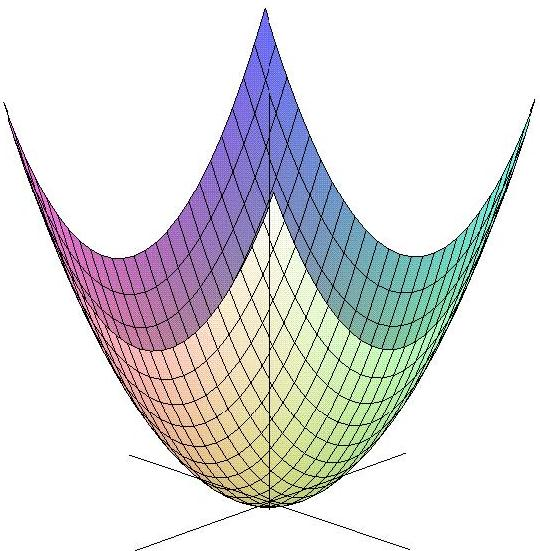
\includegraphics[width= 0.7 \textwidth,height=0.29
\textheight]{unid1graf23.jpg}
\end{center}
\caption{$f(x,y) = x^2 + y^2$}\label{Figura20}
\end{figure}

\end{ejemplo}


\begin{ejemplo}
Encuentre todos los puntos cr\'{\i}ticos  de la funcion $f(x,y) =
12x - x^3 - 4y^2$ y clasifique cada uno como un m\'aximo relativo,
un m\'{\i}nimo relativo o un punto silla.

\textbf{Soluci\'on}

Como
\[
  f_x = 12- 3x^2 \quad  \text{y} \quad f_y = -8y
\]

los puntos cr\'{\i}ticos  se encuentran resolviendo simultaneamente
las dos ecuaciones
\begin{align*}
  12 - 3x^2 &= 0 \\
   -8y & = 0
\end{align*}

De la segunda ecuaci\'on obtenemos $y =0$ y, de la primera,
\begin{align*}
    3x^2  &= 12 \\
    x  &= 2  \  \text{o}  \ -2
\end{align*}

Por tanto, hay dos puntos cr\'{\i}ticos, $(2,0)$ y $(-2,0)$.

Para determinar la naturaleza de estos puntos, primero se calcula
\[
     f_{xx} = -6x   \quad f_{yy} = -8  \quad  \text{y} \quad f_{xy} = 0
\]

y luego se forma la funci\'on
\[
     D =  f_{xx}f_{yy} - (f_{xy})^2  = (-6x)(-8) - 0 = 48x
\]

Al aplicar la prueba de las segundas derivadas parciales a los dos
puntos cr\'{\i}ticos, se obtiene
\[
   D(2,0) = 48(2) = 96 > 0  \quad \text{y} \quad f_{xx}(2,0) = -6(2)
   = -12< 0
\]

y
\[
  D(-2,0) = 48(-2) = -96 < 0
\]

de modo que hay un m\'aximo realtivo en $(2,0)$ y un punto silla en
$(-2,0)$. Ver figura 22.

\begin{figure}[h]
\begin{center}
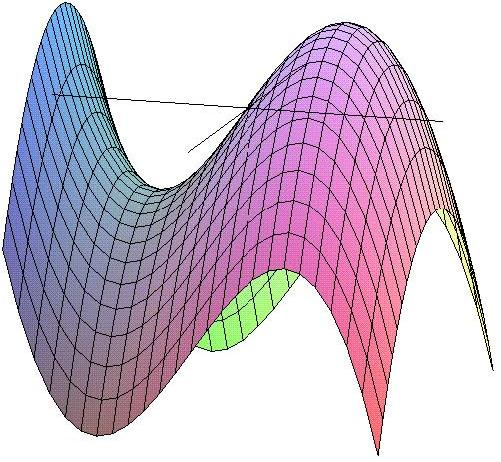
\includegraphics[width= 0.7 \textwidth,height=0.29
\textheight]{unid1graf24.jpg}
\end{center}
\caption{$f(x,y) = 12x - x^3 - 4y^2$}\label{Figura16}
\end{figure}
\end{ejemplo}

\begin{ejemplo}
Encuentre todos los puntos cr\'{\i}ticos de la funci\'on $f(x,y) =
x^3 - y^3 + 6xy$ y clasifique cada uno como m\'aximo relativo,
m\'{\i}nimo relativo o punto silla.

\vspace{.2cm}

\textbf{Soluci\'on}

Como
\[
    f_x = 3x^2 + 6y  \quad  \text{y} \quad  f_y = -3y^2 + 6x
\]

los puntos cr\'{\i}ticos de $f$ se encuentran resolviendo
simult\'aneamente las dos ecuaciones

\[
   3x^2 + 6y = 0  \quad   \text{o}  \quad  -3y^2 + 6x = 0
\]

De la primera ecuaci\'on se obtiene $y = -\frac{x^2}{2}$ que se
puede sustituir en la segunda ecuaci\'on para encontrar

\begin{align*}
  -3 \left( \frac{-x^2}{2} \right)^2 + 6x &= 0 \\
  -\frac{3x^4}{4} +  6x &= 0 \\
  -x(x^3 - 8) &= 0
\end{align*}

Las soluciones de dicha ecuaci\'on  son $x = 0$ y $x = 2$. Estas son
las coordenadas $x$ de los puntos cr\'{\i}ticos  de $f$. Para
obtener las coordenadas $y$ correspondientes, sustituya estos
valores de $x$ en la ecuaci\'on $y = - \frac{x^2}{2}$ (o en
cualquiera de las dos ecuaciones originales).

\vspace{.2cm}

As\'{\i} encontrara que $y = 0$ cuando $x = 0$ y $y = -2$ cuando $x
= 2$. De ah\'{\i} se deduce que los puntos cr\'{\i}ticos de $f$ son
$(0,0)$ y $(-2,2)$.

\vspace{.2cm}

Las derivadas parciales de segundo orden de $f$
 son
 \[
   f_{xx} = 6x \quad  f_{yy} = -6y  \quad \text{o}  \quad f_{xy} = 6
  \]
Por tanto,
\[
  D(x,y) = f_{xx} f_{yy} - (f_{xy})^2 = -36xy -36 =  -36(xy + 1)
\]

Como
\[
   D(0,0) = -36[(0)(0) + 1] = -36 < 0
\]

se deduce que $f$ tiene un punto silla en $(0,0)$. Como
\[
    D(2,-2)= -36 [2(-2) + 1] = 108 > 0
\]
y
\[
  f_{xy}(2,-2) = 6(2)= 12 > 0
\]

se ve que $f$ tiene un m\'{\i}nimo relativo en $(2,-2)$.

\end{ejemplo}


\begin{ejemplo}
Sea $Y = F(K,L)$ es una funci\'on de producci\'on,  donde $K$ es el
capital y $L$ es el trabajo. Designemos por $p$ el precio por unidad
de producci\'on, por $r$ el costo por unidad de capital y $w$ el
precio (o tasa de salario) por unidad de trabajo. El beneficio de
producir y vender $F(K,L)$ unidades es entonces:
\[
   \pi(K,L)= pF(K,L) -rK - wL,
\]
Si $F$ es diferenciable y $\pi$ tiene un m\'aximo con $K> 0$ y $L >
0$, entonces por el teorema (\ref{porden})
 las parciales de $\pi$ deben anularse. Por tanto, las
condicione de primer orden son:
\begin{align*}
   \pi'_K(K,L) &= p F_{K}'(K,L)- r = 0 \\
   \pi'_L(K,L) &= p F_{L}'(K,L)- w = 0.
\end{align*}
As\'{\i} una condici\'on necesaria para que el beneficio tenga un
m\'aximo para $K = K^{*}$ y $L = L^{*}$ es que:
\[
  pF_{K}'(K^{*}, L^{*})= r, \, \,  pF_{L}(K^{*}, L^{*}) = w
\]

otra forma de interpretarlo es
\[
  F_{K}'(K^{*}, L^{*})= \frac{r}{p}, \, \,  F_{L}(K^{*}, L^{*}) =
  \frac{w}{p}
\]

Supongamos que incrementamos el capital en una unidad desde el
ni\-vel $K^{*}$. \textquestiondown Cu�nto ganaremos? La producci\'on
crece en, aproximadamente, $F_{K}'(K^{*},L^{*})$ unidades. Como cada
una de esas unidades tiene un precio $p$, el aumento de ingresos es
de $p F_{K}'(K^{*}, L^{*})$ aproximadamente.\textquestiondown
C\'uanto se pierde en este aumento unitario de capital? Se pierde
$r$, que es el costo de una unidad de capital. Estas dos cantidades
deben ser iguales. La segunda ecuaci\'on tiene una interpretaci\'on
an\'aloga: incrementando el trabajo  en una unidad desde el nivel
$L^{*}$ se tendr\'a un aumento aproximado de los ingresos  de $p
F_{L}'(K^{*}, L^{*})$, mientras que el costo del trabajo extra es
$w$, y esas dos cantidades son iguales. El punto $(K^{*}, L^{*})$
que maximiza el beneficio tiene la propiedad de que el ingreso extra
generado por un aumento unitario de capital o trabajo se compensa
con el aumento del costo.
\end{ejemplo}


\begin{problema}
Supongamos que:
\[
   Y = F(K,L) =  6 K^{\frac{1}{2}} L^{\frac{1}{3}},
\]
es una funci\'on de producci\'on,  donde $K$ es el capital y $L$ es
el trabajo. Sean $p = 0.5$ el precio por unidad de producci\'on, $r
= 0.1$ el costo por unidad de capital y $w = 1$ el precio por unidad
de trabajo. Hallar el beneficio m\'aximo en este caso.
\end{problema}


\textbf{Soluci\'on del problema 13:} La funci\'on de beneficios es:
\[
   \pi(K,L)= 0.5 \cdot    6 K^{\frac{1}{2}} L^{\frac{1}{3}} - 0.1 K -
  1 \cdot L = 3 K^{\frac{1}{2}} L^{\frac{1}{3}} - 0.1 K - L,
\]
Las condiciones de primer orden son:
\begin{align*}
   \pi'_K(K,L) &= 1.5 \cdot  K^{-\frac{1}{2}} L^{\frac{1}{3}} - 0.1 = 0, \\
   \pi'_L(K,L) &=   K^{\frac{1}{2}} L^{-\frac{2}{3}} - 1  =  0.
\end{align*}

La primera ecuaci\'on da $K ^{-1/2} = L^{1/3}$. Sustitutendo este
valor de $K^{\frac{1}{2}}$ en la segunda ecuaci\'on obtenemos $15
L^{\frac{1}{3}} L^{-\frac{2}{3}} = 1$. As\'{\i}  $15
L^{-\frac{1}{3}} = 1$,
 \'o $L = 15^{3}$. Veamos que el punto estacionario $(K,L) = (50.625, 3.375)$ maximiza los
 beneficios.

\vspace{.2cm}

 Tenemos que:
 \[
  \pi(K,L) = 3 K^{\frac{1}{2}} L^{\frac{1}{3}} - 0.1 k - L,
 \]
 con $K > 0$ y $L > 0$, luego:
 \begin{align*}
   \pi_{KK}'' &= -\frac{3}{4} K^{-3/2} L^{1/3} \, \pi_{KL}'' = \frac{1}{2} K^{-1/2} L^{-2/3}, \text{y} \\
   \pi_{LL}'' &= -\frac{2}{3} K^{1/2} L^{-5/3}.
\end{align*}
Por tanto, $\pi_{KK}'' < 0$ y $\pi_{LL}'' < 0 $ para todo $K > 0$ y
$L > 0$. Adem\'as,
\[
  \pi_{KK}''\pi_{LL}'' - (\pi_{KL}'')^{2} = \frac{1}{2} K^{-1} L^{-4/3} -
  \frac{1}{4} K^{-1} L^{-4/3} > 0
\]
Por el teorema \ref{soptimos} el punto $(50.625, 3.375)$ es un m\'aximo de
$\pi(K,L)$. Entonces, para maximizar los beneficios, hay que tomar:
\begin{equation*}
     L = 15^{3} = 3.375 \,\, \text{y} \,\, K = 15^{2}L^{2/3}
     = 15^{4} = 50.625
\end{equation*}
El valor de la funci\'on de beneficios es $\pi(50.625, 3.375) =
1687.5$.

\newpage

\setcounter{page}{1}

\begin{center}
\textbf{TAREA 1: OPTIMIZACI\'ON LIBRE EN VARIAS VARIABLES}
\end{center}

Trabajo en equipos con dos o tres integrantes.

\vspace{.3cm}

En los ejercicios 1 a 6, encontrar los valores m\'aximos,
m\'{\i}nimos o puntos de silla de cada funci\'on.
\begin{enumerate}
\item $f(x,y) = -2x^2 - 2xy - 2y^2 + 36x + 42y -158$ \vspace{.2cm}
\item $f(x,y) = x^2  + y^2 - 6x + 8y + 35$ \vspace{.2cm}
\item $f(x,y) = x^3 + y^3 + 3xy$ \vspace{.2cm}
\item $f(x,y) = -2x^2 - y^2 + 4x + 4y -3$ \vspace{.2cm}
\item $f(x,y) = x^2  + xy  + y^2 - 3x + 2$ \vspace{.2cm}
\item $f(x,y) = 4x^3 + y^3 -12x  -3y $ \vspace{.2cm}
\end{enumerate}

\newpage

\setcounter{page}{1}

\subsection{Optimizaci�n restringida}
\textbf{El M\'etodo de los multiplicadores de Lagrange}
\medskip

Las variables que aparecen en los problemas econ\'omicos  de
optimizaci\'on  estan casi siempre sometidas a ciertas
restricciones. Por ejemplo, precios y cantidades son a menudo no
negativos por definici\'on, y la escasez impone que las cantidades
que se consumen est\'en acotadas superiormente. Adem\'as cuotas de
producci\'on, limitaciones presupuestarias y otras condiciones
pueden restringir el rango de elecci\'on.

\vspace{.2cm} Cuando la restricci\'on es una funci\'on complicada, o
cuando hay todo un sistema de ecuaciones para expresar
restricciones, los economistas usan el \textbf{ m\'etodo de los
multiplicadores de Lagrange}.
\medskip


Para hallar las soluciones del problema:

\begin{equation}
\label{principal}
   \max(\min) \, \, f(x,y) \mbox{ sujeta a }  g(x,y) = c
\end{equation}

se usa el m\'etodo de los multiplicadores de Lagrange  el cual consiste en:

\begin{enumerate}
   \item Escribir la funci\'on lagrangiana:
  \[
    \mathcal{L}(x,y) =  f(x,y) - \lambda (g(x,y) - c)
  \]
 donde $\lambda$ es una constante.
 \vspace{.2cm}
   \item Derivar $\mathcal{L}$ con respecto a $x$ e $y$, e igualar a cero las parciales.
   \vspace{.2cm}
  \item  Escribir el sistema formado por las dos ecuaciones de 2 junto con la restricci\'on:
\begin{align*}
      f_1'(x,y) &= \lambda g_1'(x,y) \\
      f_2'(x,y) &= \lambda g_2'(x,y) \\
      g(x,y) &= c
\end{align*}
  \item Resolver esas tres ecuaciones en las tres inc\'ognitas $x$, $y$ y $\lambda$.
\end{enumerate}

Consideremos el problema:
\[
\max \, \, f(x,y) \mbox{ sujeta a }  g(x,y) = c
\]
Sean $x^{*}$ e $y^{*}$ los valores de $x$ y $y$ que resuelven el
problema. En general $x^{*}$ y $y^{*}$ dependen de $c$. Vamos a
suponer que $x^{*} = x^{*}(c)$ e $y^{*} = y^{*}(c)$ son funciones
diferenciables de $c$. Entonces:
\[
 f^{*}(c)= (x^{*}(c), y^{*}(c)),
\]
es tambi\'en funci\'on de $c$. A $f^{*}(c)$ se le llama
$\textbf{funci\'on valor \'optimo}$ para el problema. Cuando se usa
el m\'etodo lagrangiano, el valor correspondiente del multiplicador
de Lagrange tambi\'en depende de $c$. Si se satisfacen ciertas
condiciones de regularidad tenemos el siguiente resultado:
\begin{equation}\label{a}
    \frac{df^{*}(c)}{dc} =  \lambda(c)
\end{equation}
As\'{\i} el multiplicador de Lagrange $\lambda = \lambda(c)$ es la
tasa de variaci\'on del valor \'optimo de la funci\'on objetivo
cuando la constante de restricci\'on $c$ cambia.
\vspace{.2cm}


\begin{teorema}
\label{Lagrange}
(Teorema de Lagrange) Supongamos que $f(x,y)$ y $g(x,y)$ tienen derivadas parciales continuas en
un dominio $A$ del plano $xy$ y que $(x_0,y_0)$ es un punto interior
de $A$ y un \'optimo local para $f(x,y)$ sujeta a la restricci\'on
$g(x,y) = c$. Supongamos adem\'as que no se anulan a la vez
$g_1'(x_0,y_0)$ y $g_2'(x_0,y_0)$. Existe un n\'umero \'unico
$\lambda$ tal que la funci\'on lagrangiana:
\[
    \mathcal{L}(x,y) =  f(x,y) - \lambda (g(x,y) - c)
\]
tiene un punto estacionario en $(x_0,y_0)$.
\end{teorema}

Bajo las hip\'otesis del Teorema \ref{Lagrange} el m\'etodo de los multiplicadores de Lagrange
para el problema:
\[
   \max(\min) \, \, f(x,y) \mbox{ sujeta a }  g(x,y) = c
\]
da condiciones necesarias para la soluci\'on del problema. El siguiente resultado da condiciones suficientes
para resolver el problema.

\begin{teorema}
\label{slag}
(Suficiencia global) Supongamos que las funciones $f(x,y)$ y $g(x,y)$ son
continuamente diferenciables en un conjunto abierto convexo $A$ de
$\Bbb{R}^{2}$ y sea $(x_0,y_0) \in A$ un punto estacionario para la
funci\'on lagrangeana:
\[
    \mathcal{L}(x,y) =  f(x,y) - \lambda (g(x,y) - c)
\]
Supongamos adem\'as que $g(x_0,y_0) = c$. Entonces:
\begin{enumerate}
  \item $\mathcal{L}$ es concava $\Longrightarrow$ resuelve el problema de maximizaci\'on de ($\ref{principal}$).
  \item $\mathcal{L}$ es convexa $\Longrightarrow$ resuelve el problema de minimizaci\'on de ($\ref{principal}$).
\end{enumerate}
\end{teorema}

\begin{problema}
Empleando $L$ unidades de mano de obra y $K$ unidades de capital,
una empresa puede elaborar $Q$ unidades de su producto, con
\[
  Q= F(L,K) = 50 L^{2/3} K^{1/3}
\]

Le cuesta a la empresa \$100 por cada unidad de mano de obra y \$300
por cada unidad de capital empleado. La empresa dispone de una suma
de \$45,000 para prop�sitos de producci�n.

\begin{enumerate}
 \item[i)] Mediante el m�todo de multiplicadores de Lagrange
 determine las unidades de mano de obra y de capital que la empresa
 deber�a utilizar con objeto de maximizar su producci�n.
 \item[ii)] Gr�fique a trav�s de las curvas de nivel los resultados
 obtenidos.
\end{enumerate}
\end{problema}

\textbf{Soluci\'on del problema 14}

\begin{enumerate}
\item[i)] Aqu� la funci�n a maximizar es
\[
    \max Q(L,K) = 50 L^{2/3} K^{1/3}
\]

El costo de emplear $L$ unidades de mano de obra a \$100 cada una y
$K$ unidades de capital a \$300 cada una es de $(100L+300K)$ pesos.
Puesto que deseamos disponer por completo de la suma de \$45 000,
debemos tener que

\[
100L+300K=45,000
\]

Maximizaremos $Q(L,K)$ sujeta a esta restricci�n. La funci�n
lagrangeana es
\[
\mathcal{L}(L,K,\lambda)= 50 L^{2/3} K^{1/3}- \lambda (100L+300K -
45,000).
\]

A fin de obtener un m�ximo de $Q(L,K)$, debe cumplirse que:
\begin{align*}
\frac{\partial \mathcal{L}}{\partial L} &=
\frac{100}{3}L^{-1/3}K^{1/3}-100 \lambda=0 \\[.3cm]
\frac{\partial \mathcal{L}}{\partial K} &=
\frac{50}{3}L^{2/3}K^{-2/3}-300 \lambda=0 \\[.3cm]
\frac{\partial \mathcal{L}}{\partial \lambda} &=
-(100L+300K-45,000)=0
\end{align*}

Resolviendo las primeras dos ecuaciones para $\lambda$, obtenemos
\[
\lambda = \frac{1}{3} L^{-1/3} K^{1/3} \,\,\,\, \text{y} \,\,\,\,
\lambda = \frac{1}{18} L^{2/3} K^{-2/3}
\]

Ahora igualamos los dos valores de $\lambda$
\[
\frac{1}{3} L^{-1/3} K^{1/3} = \frac{1}{18} L^{2/3} K^{-2/3}
\]

Despejando en ambos lados $L$, obtenemos
\[
L = 6K
\]

Sustituyendo esto en la expresi�n de $\frac{\partial
\mathcal{L}}{\partial \lambda}$ resulta que

\[
600K+300K-45,000=0 \,\,\,\, \text{o bien} \,\,\,\, K=50
\]

Por consiguiente, $L=6K=300$ y la empresa maximiza su producci�n si
emplea 300 unidades de mano de obra y 50 de capital.
\item[ii)] La gr�fica de las curvas de nivel se muestra en la
figura 23.
\end{enumerate}

\begin{figure}[h]
\begin{center}
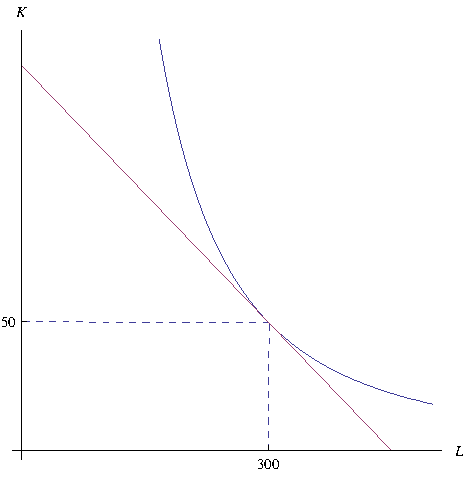
\includegraphics[width= 0.7 \textwidth,height=0.29
\textheight]{unid1graf29.pdf}
\end{center}
\caption{$50 L^{2/3} K^{1/3}$ sujeto a $100L+300K =
45,000$}\label{Figura22}
\end{figure}

\begin{problema}
Un consumidor tiene \$600 para gastar en dos mercancias, la primera
de las cuales cuesta \$20 por unidad y, la segunda, \$30 por unidad.
Suponga que la utilidad obtenida por el consumidor con $x$ unidades
de la primera mercanc�a y $y$ unidades de la segunda mercanc�a, est�
dada por la \textbf{funci�n de utilidad de Cobb-Douglas} $U(x,y)=
10x^{3/5}y^{2/5}$.

\begin{enumerate}
 \item[i)] Mediante el m�todo de multiplicadores de Lagrange
 determine las unidades de cada mercanc�a que debe comprar el
 consumidor para maximizar su utilidad.
 \item[ii)] Gr�fique a trav�s de las curvas de nivel los resultados
 obtenidos.
\end{enumerate}
\end{problema}

\textbf{Soluci�n al problema 15}
\medskip

\begin{enumerate}
\item[i)] Aqu� la funci�n a maximizar es
\[
    \max U(x,y) = 10 x^{3/5} y^{2/5}
\]

El costo total de comprar $x$ unidades de la primera mercanc�a a
\$20 por unidad y, $y$ unidades de la segunda mercanc�a a \$30 por
unidad, es $20x+30y$. Como el consumidor tiene s�lo \$600 para
gastar, la meta es maximizar la utilidad $U(x,y)$ sujeta a la
restricci�n presupuestal
\[
20x+30y=600
\]

Maximizaremos $U(x,y)$ sujeta a esta restricci�n. La funci�n
lagrangeana es
\[
\mathcal{L}(x,y,\lambda)= 10 x^{3/5} y^{2/5}- \lambda (20x+30y -
600).
\]

A fin de obtener un m�ximo de $U(x,y)$, debe cumplirse que:
\begin{align*}
\frac{\partial \mathcal{L}}{\partial x} &=
6 x^{-2/5} y^{2/5}-20 \lambda=0 \\[.3cm]
\frac{\partial \mathcal{L}}{\partial y} &=
4 x^{3/5} y^{-3/5}-30 \lambda=0 \\[.3cm]
\frac{\partial \mathcal{L}}{\partial \lambda} &= -(20x+30y-600)=0
\end{align*}

Resolviendo las primeras dos ecuaciones para $\lambda$, obtenemos
\[
\lambda = \frac{3}{10} x^{-2/5} y^{2/5} \,\,\,\, \text{y} \,\,\,\,
\lambda = \frac{2}{15} x^{3/5} y^{-3/5}
\]

Ahora igualamos los dos valores de $\lambda$
\[
\frac{3}{10} x^{-2/5} y^{2/5} = \frac{2}{15} x^{3/5} y^{-3/5}
\]

Despejando en ambos lados $y$, obtenemos
\[
y = \frac{4}{9}x
\]

Sustituyendo esto en la expresi�n de $\frac{\partial
\mathcal{L}}{\partial \lambda}$ resulta que
\[
20x+30(\frac{4}{9}x)=600 \,\,\,\, \text{o bien} \,\,\,\, x=18
\]

Por consiguiente, $y = \frac{4}{9}(18)=8$. Esto es, para maximizar
la utilidad, el consumidor debe comprar 18 unidades de la primera
mercanc�a y 8 unidades de la segunda.

\item[ii)] La gr�fica de las curvas de nivel se muestran en la
figura 24
\end{enumerate}

\begin{figure}[h]
\begin{center}
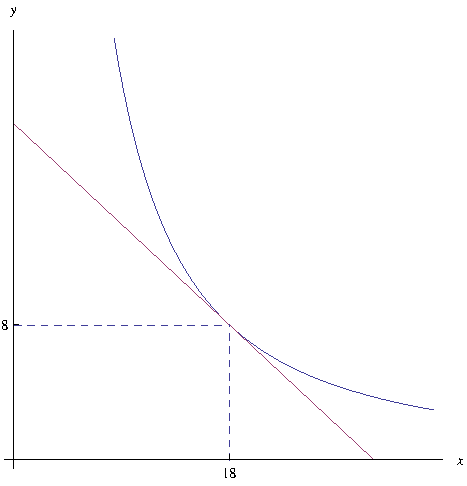
\includegraphics[width= 0.7 \textwidth,height=0.29
\textheight]{unid1graf30.pdf}
\end{center}
\caption{$10 x^{3/5} y^{2/5}$ sujeto a $20x+30y =
600$}\label{Figura23}
\end{figure}

\begin{problema}
Una empresa usa cantidades $K$ y $L$ de capital y trabajo,
res\-pec\-ti\-va\-men\-te para producir una cantidad $Q$ de un solo
producto, siguiendo la funci\'on de producci\'on:
\[
 Q = F(K,L) = K^{1/2} L^{1/4}.
\]
Los precios de capital y trabajo son $r$ y $w$ respectivamente.
\begin{enumerate}
 \item[i)] Hallar las cantidades $K$ y $L$ que  minimizan los costos, as\'{\i} como el
costo m\'{\i}nimo, como funciones de $r$, $w$ y $Q$. Designemos por
$K^{*}$, $L^{*}$, y $C^{*}$ a estos valores.
 \item[ii)] Comprobar que:
\[
   K^{*} = \frac{\partial C^{*}}{\partial r}, \, L^{*} = \frac{\partial C^{*}}{\partial w}, \,
   \lambda = \frac{\partial C^{*}}{\partial Q}, \,  \frac{\partial K^{*}}{\partial w} = \frac{\partial L^{*}}{\partial r}.
\]
\end{enumerate}

\end{problema}
\textbf{Soluci\'on del problema 16}
\begin{enumerate}
\item[i)] La empresa tiene que resolver el siguiente problema de minimizaci\'on de costo:
\[
    \min C = rK + wL \mbox{ sujeta  a } Q = K^{1/2} L^{1/4}
\]
La funci\'on lagrangiana es:
\[
\mathcal{L}(K,L)= rK  + wL - \lambda (K^{1/2} L^{1/4} - Q).
\]
Igualando las derivadas parciales a cero obtenemos:
\begin{align*}
  \frac{\partial \mathcal{L}}{\partial K} &= r - \frac{1}{2} \lambda K^{-1/2} L^{1/4} = 0, \\
\frac{\partial \mathcal{L}}{\partial L} &= w - \frac{1}{4} \lambda
K^{1/2} L^{-3/4} = 0.
\end{align*}
As\'{\i}, $r = \frac{1}{2} \lambda K^{-1/2} L^{1/4}$ y $w =
\frac{1}{4} \lambda K^{1/2} L^{-3/4}$. Despejando $\lambda$ de estas
dos ecuaciones e igualando los resultados:
\[
\lambda = 2r \lambda K^{1/2} L^{-1/4} = 4w K^{-1/2}L^{3/4}
\]

Simplificando por $K^{1/2} L^{1/4}$ obtenemos $2rK = 4wL$, luego $L
= (r/2w)K$. Llevando este valor a la restricci\'on $K^{-1/2} L^{1/4}
= Q$ tenemos que $K^{1/2}(r/2w)^{1/4} K^{1/4} = Q$, luego:

\begin{equation}
\label{soluc}
 K^{3/4} = 2^{1/4}r^{-1/4} w^{1/4}Q
\end{equation}


Elevando ambos miembros de la igualdad (\ref{soluc}) a $4/3$ y
usando super\'{\i}ndices ($*$) se tiene:
\[
 K^{*} = 2^{1/3}r^{-1/3} w^{1/3}Q^{4/3}
\]
y as\'{\i}:
\[
L^{*} = (r/2w) K^{*} = 2^{-2/3}r^{2/3} w^{-2/3}Q^{4/3}
\]
La funci\'on lineal $r K + w L$  es convexa y la funci\'on  de
Cobb-Douglas $K^{1/2} L^{1/4}$ es c\'oncava. Como $\lambda \geq 0$,
la funci\'on lagrangiana:
\[
\mathcal{L}(K,L)= rK  + wL + (-\lambda) (K^{1/2} L^{1/4} - Q)
\]
es suma de dos funciones convexas y, por tanto, es convexa. Por el
Teorema \ref{slag}, el punto $(K^{*}, L^{*})$ minimiza el costo. El costo m\'{\i}nimo
correspondiente  es:
\begin{equation}
\label{soluc2}
   C^{*} = rK^{*} + wL^{*} = 3 \cdot 2^{-2/3}r^{2/3} w^{1/3}Q^{4/3}
\end{equation}
Finalmente, usando $(\ref{soluc})$
 otra vez, hallamos  $\lambda = 2^{4/3}r^{2/3} w^{1/3}Q^{1/3}$.
 \vspace{.2cm}
\item[ii)] Por (\ref{soluc2}) tenemos que:
\begin{align*}
  \frac{\partial C^{*}}{\partial r} &= 3 \cdot 2^{- 2/3} \frac{2}{3} r^{-1/3} w^{1/3}Q^{4/3} \\
   &=  2^{1/3}r^{-1/3} w^{1/3}Q^{4/3} \\
   &= K^{*}
\end{align*}
 Observemos que la tercera igualdad de ii) es un caso particular de (\ref{a}), y vemos que el
valor com\'un es $\lambda = \partial C^{*}/ \partial Q =
2^{4/3}r^{2/3} w^{1/3}Q^{1/3}$. Se comprueban f\'acilmente las
dem\'as igualdades.
\end{enumerate}

\newpage

\setcounter{page}{1}

\begin{center}
\textbf{TAREA 2: OPTIMIZACI\'ON RESTRINGIDA}
\end{center}

Trabajo en equipo con dos o tres integrantes.

\begin{enumerate}
\item Emplendo $K$ unidades de capital y $L$ unidades de mano de
obra, una empresa puede elaborar $Q$ unidades de su producto, con
\[
    Q(K,L) = 50 K^{\frac{1}{3}} L^{\frac{2}{3}}
\]
Le cuesta a la empresa \$300 por cada unidad de capital y \$100  por
cada unidad de mano de obra empleado. La empresa dispone de una suma
de  \$ 45,000 para propositos de producci\'on.
\begin{enumerate}
  \item Mediante el m\'etodo de multiplicadores de Lagrange
  determine las unidades de capital y trabajo que la empresa
  deber\'{\i}a  utilizar con objeto de maximizar su producci\'on.
  \item Grafique las curvas de nivel de la funci\'on de
  restricci\'on presupuestaria y de la funci\'on de producci\'on.
\end{enumerate}

\item Emplendo $K$ unidades de capital y $L$ unidades de mano de
obra, una empresa puede elaborar $Q$ unidades de su producto, con
\[
    Q(K,L) = 12 K^{\frac{2}{5}} L^{\frac{2}{5}}
\]
Le cuesta a la empresa \$40 por cada unidad de capital y \$5  por
cada unidad de mano de obra empleado. La empresa dispone de una suma
de  \$ 800 para propositos de producci\'on.
\begin{enumerate}
  \item Mediante el m\'etodo de multiplicadores de Lagrange
  determine las unidades de capital y trabajo que la empresa
  deber\'{\i}a  utilizar con objeto de maximizar su producci\'on.
  \item Grafique las curvas de nivel de la funci\'on de
  restricci\'on presupuestaria y de la funci\'on de producci\'on.
\end{enumerate}

\item Supongamos que tenemos dos bienes con unos precios de $p_1 = 2$
y $p_2 = 5$, con un ingreso $m =40$ y una funci\'on de utilidad:
\[
   u(x,y) = x^\frac{1}{3} y^{\frac{1}{2}}
\]
\begin{enumerate}
   \item Mediante el m\'etodo de multiplicadores de Lagrange
   determine las unidades del bien uno y del bien dos que el
   consumidor deber\'{\i}a utilizar con objeto de maximizar su
   utilidad.
   \item Grafique las curvas de nivel de la funci\'on de
   restricci\'on presupuestaria  y de la funci\'on de utilidad.
\end{enumerate}

\item Supongamos que tenemos dos bienes con unos precios de $p_1 = 20$
y $p_2 = 5$, con un ingreso $m =600$ y una funci�n de utilidad:
\[
   u(x,y) = 40x^\frac{1}{2} y^{\frac{1}{2}}
\]
\begin{enumerate}
   \item Mediante el m\'etodo de multiplicadores de Lagrange
   determine las unidades del bien uno y del bien dos que el
   consumidor deber\'{\i}a utilizar con objeto de maximizar su
   utilidad.
   \item Grafique las curvas de nivel de la funci\'on de
   restricci\'on presupuestaria  y de la funci\'on de utilidad.
\end{enumerate}
\end{enumerate}

\end{document}
